\subsection{Änderungsverlauf}
\begin{table}[h]
    \centering
    \begin{tabular}{|c|c|c|p{7cm}|}
        \hline
        \textbf{Version} & \textbf{Datum} & \textbf{Autor} & \textbf{Änderungen} \\ \hline
        1.0 & 27.01.2025 & M. Lauterbach & Initialer Stakeholder-Kontakt und Grundanforderungen definiert \\ \hline
        1.1 & 22.02.2025 & M. Lauterbach & TELOS-Machbarkeitsstudie erstellt \\ \hline
        1.2 & 03.03.2025 & M. Lauterbach & Dokumentationsstruktur etabliert \\ \hline
        1.3 & 05.03.2025 & M. Lauterbach & Sprachliche Überarbeitung und Korrekturen \\ \hline
        1.4 & 10.03.2025 & M. Lauterbach & Choreographie-spezifische Anforderungen (FA-07 bis FA-12) integriert \\ \hline
        1.5 & 30.03.2025 & M. Lauterbach & Visual-Design-Anforderungen nach Stakeholder-Feedback erweitert \\ \hline
        1.6 & 17.04.2025 & M. Lauterbach & Restriktive Präzisierung der Anforderungen basierend auf finalen Visual-Spezifikationen für Systemintegration \\ \hline
    \end{tabular}
    \caption{Dokumentations-Changelog}
    \label{tab:changelog}
\end{table}

\subsubsection{Technische Infrastruktur der Filmakademie}
\begin{itemize}
    \item \textbf{Hardware:} NVIDIA RTX 3080, AMD Ryzen 9750
    \item \textbf{Software:} TouchDesigner 2023.11
    \item \textbf{Tracking:} Kinect V2 mit RGB- und Tiefensensor
    \item \textbf{Studiodimensionen:} 383 m² (21m × 15m)
\end{itemize}

\begin{figure}[htbp]
    \centering
    \adjustbox{max width=0.9\textwidth, max height=0.8\textheight, keepaspectratio}{%
        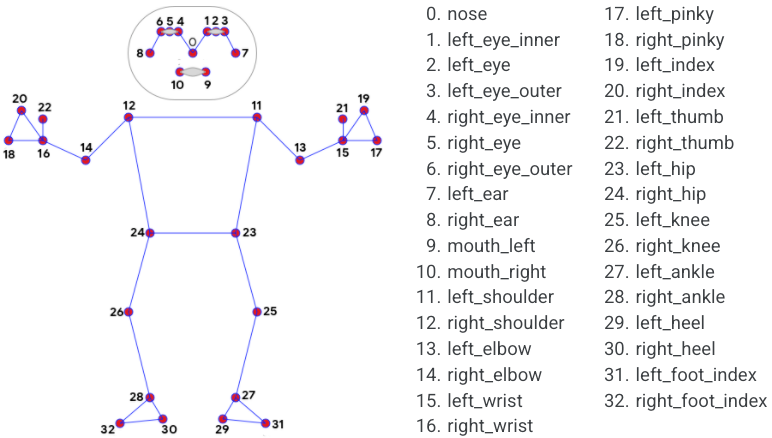
\includegraphics{images/docupictures/mediapipeNODES.png}%
    }
    \caption{MediaPipe Skeleton-Nodes, die die Basis für die Skelett-Visualisierung bilden}
    \label{fig:mediapipe_nodes}
\end{figure}

\subsection{Funktionale Anforderungen}

\textbf{Kern-Tracking-Funktionalität:}
\begin{itemize}
    \item \textbf{FA-01:} Einfachpersonen-Erkennung und -Verfolgung im Kinect-Sichtfeld
    \item \textbf{FA-02:} Echtzeit-Verarbeitung der Positionsdaten für regelbasierte Trigger
    \item \textbf{FA-05:} Native TouchDesigner-Integration für Visualisierungssteuerung
    \item \textbf{FA-06:} Modulare Systemarchitektur für iterative Optimierung
\end{itemize}

\textbf{Performance-spezifische Anforderungen:}
\begin{itemize}
    \item \textbf{FA-07:} Boolean-Node-Triggering/Switch-Triggers und Python-basierte Eigenschaftsmanipulation
    \item \textbf{FA-08:} Personen-Eintrittserkennung mit automatischer Aktivierung
    \item \textbf{FA-09:} Selektives Single-Person-\\Tracking (Kameramann-Ausblendung)
\end{itemize}

\textbf{Projections-Mapping-Funktionalität:}
\begin{itemize}
    \item \textbf{FA-11:} Beamer-Kinect-Kalibrierung für präzise Performer-Ausblendung/Hervorhebung
    \item \textbf{FA-14:} Relative 2D-Positionierung der Visuals zum Performer
\end{itemize}

\textbf{Choreographie-spezifische Visualisierungslogik:}
\begin{itemize}
    \item \textbf{FA-16:} Extremitäten-responsive Blitzeffekte mit radialer Positionierung
    \item \textbf{FA-17:} Hockbewegung-getriggerte Umrandungseffekte bei kreisförmigen Visuals
\end{itemize}